\chapter{Experiments and analysis}
\section{Experiment 1: Transitivity ratios}\label{sec:exp1}
\subsection{Background: Verb transitivity}
If we were to take a top-down approach to the task of verb classification, i.e., to categorize verbs of a language into verb classes according to their syntacto-semantic properties and behavior, we could well imagine ourselves with fine-grained verb classes à la \citet{levin1993} in the end, but will likely have to start with more basic distinctions and, first among them, that of verb \textit{transitivity}. 

In comparison with the more intricate distinctions made in valency typology, the notion of \textit{transitivity}, i.e., whether a verb can take one or more objects, is probably familiar to any of us who has been in a foreign language classroom. Traditionally, a binary distinction is made between \textit{intransitive} verbs, which take only a subject and no objects and \textit{transitive} verbs, which take one or more objects. A categorical approach would then subdivide the verbs into further categories including \textit{ditransitive} verbs (those taking two objects), ambitransitive verbs (those that can be used both transitively and intransitively), etc.

\todo{semantic aspects of transitivity}

From a functionalist perspective, however, the categorical distinctions often fail to capture other important aspects of how verbs are used. A telling early corpus-based study \citep{biber1998} touches upon this when comparing the English verbs \textit{begin} and \textit{start}. At first glance, English appears to have provided us with two verbs that are not only semantically synonymous but share valency properties as well, as they can both be used in transitive and intransitive constructions:

\begin{exe}
\ex\label{example-begin_start}
  \begin{xlist}
  \ex{I had better issue a survival kit before we \textit{start}/\textit{begin}.\\ \strut\hfill \textbf{intransitive}}
  \ex{Then they \textit{started}/\textit{began} the quota system.\\ \strut\hfill \textbf{transitive with noun phrase}}
  \ex{They'd \textit{started}/\textit{begun} leaving before I arrived.\\ \strut\hfill \textbf{transitive with \textit{-ing} clause}}
  \ex{One of the wheels had \textit{started}/\textit{begun} to wobble.\\ \strut\hfill \textbf{transitive with \textit{to} clause}}
  \end{xlist}
\end{exe}

This however belies the different usage patterns exhibited by these verbs, as \citet[95]{biber1998} demonstrate with statistics from the British National Corpus (BNC): while both uses are present for both verbs, \textit{begin} is used more often in a transitive frame than \textit{start} across different genres: in fiction, 78\% of \textit{begin} occurrences (196/250) are with various transitive patterns vs. only 60\% for \textit{start} (149/250); transitive uses are less frequent in academic texts in general but the observation of relatively higher transitivity for \textit{begin} still holds (57\% vs. 36\%, or 110/192 vs. 51/142).

The UD annotations provide us with good facility to investigate transitivity at a lexeme-level quantitatively, as it would allow us similar insights but with a wider range of languages and better coverage of their respective verbal lexicon. The relevant dependency relations \textsc{nsubj} and \textsc{obj} are defined to cover respectively the first and second core arguments of a verb with their typical syntactic roles as subject and object. This is defined without respect to specific cases (even though typically the accusative in languages with a case system) or semantic roles (even though they would typically be the proto-agent and proto-patient) in an effort to not prejudice the scheme with a priori categories to the extent possible. The renaming of the \textsc{dobj} relation to \textsc{obj} changes introduced by UD v2 \citep{nivre2020} reflects the same effort as well.

\subsection{Experiment design}

Given the clear and typologically sound UD dependency relations, one can be forgiven for having already started up the code editor and tried to calculate the transitivity ratio based on them. On closer examination, however, we see that arriving at a clear definition of transitivity is in fact not trivial.

We consider four different definitions of a quantitative transitivity ratio within the UD annotation scheme:

\begin{enumerate}
    \item the number of verb instances with both \textsc{nsubj} and \textsc{obj} dependents, divided by the number of verb instances with an \textsc{nsubj} dependent
    \item the number of verb instances with an \textsc{obj} dependent, divided by the number of verb instances with an \textsc{nsubj} dependent
    \item the number of verb instances with an \textsc{obj} dependent, divided by the total number of verb instances
    \item the number of verb instances with an \textsc{obj} dependent, divided by the number of verb instances with either an \textsc{nsubj} or an \textsc{obj} dependent
\end{enumerate}

Def. 1 is an attempt at enforcing the definition of the transitive object as the \textit{second} core argument of the verb by excluding from calculation instances where the first core argument (i.e., subject) is not realized. This turns out counterproductive for two reasons. Firstly, this does not sit well with the focus on transitivity, as instances of verb use where the subject is not expressed are not per se evidence against the fact that the verb is taking a transitive object; secondly, this is undesirable from a typological perspective as well, as the metric would be biased against pro-drop languages where the pronouns would often be dropped when inferrable from grammar or context. \todo{an example sentence from a pro-drop language to illustrate}

Def. 2 comes as a reaction to the deficiencies of Def. 1, namely by dropping the requirement in the numerator for verbs to have an \textsc{nsubj} dependent. However, we are now left with the opposite problem if we are to account for typological variations, where pro-drop languages are likely to have a smaller denominator, resulting in an undesired higher transitivity ratio. The pendular biases tempt us to simply drop the \textsc{nsubj} requirement in the denominator too, arriving at Def. 3, which appears to be an elegant and simple solution. That is, until we realize the verb instances where both subject and object are dropped would affect the denominator, and such usage, e.g., non-predicative usage of verbs, is unlikely to be equally frequent in different languages and would therefore interfere with the cross-lingual comparability of our transitivity ratio. Taking all these potential drawbacks into consideration, we propose Def. 4 with the number of verb instances with either an \textsc{nsubj} or an \textsc{obj} dependent in the denominator. 

\begin{table}[ht]
  \centering
  \begin{tabularx}{0.5\textwidth}{cX}
  {\#} & \textbf{Definition} \\
  \hline
  1&$[+\textsc{nsubj}, +\textsc{obj}]/ [+\textsc{subj}]$ \\
  2&$[+\textsc{obj}] / [+\textsc{nsubj}]$  \\
  3&$[+\textsc{obj}] / []$\\
  4&$[+\textsc{obj}] / [+\textsc{nsubj}] \text{ or } [+\textsc{obj}]$
  \end{tabularx}
  \caption{Potential definitions of transitivity ratio considered in §\ref{sec:exp1}, represented with feature matrices}\label{tab:transitivity-defs}
\end{table}

While we have a strong case for Def. 4 being the most principled definition, we nevertheless implement all four definitions in this experiment to empirically verify our intuitions. They are also represented with feature matrices in Tab.~\ref{tab:transitivity-defs} for quick reference. For the experiment, we go through all eligible UD corpora and compile transitivity ratio statistics for each lexeme and later summarizing the transitivity ratio statistics at a language-level.

\subsection{Results}

The full results from the experiments are included in the appendices. 
\todo{most transitive languages}
\todo{least transitive languages}
\todo{areal patterns and comparison against previous studies}

\begin{figure}
  \centering
  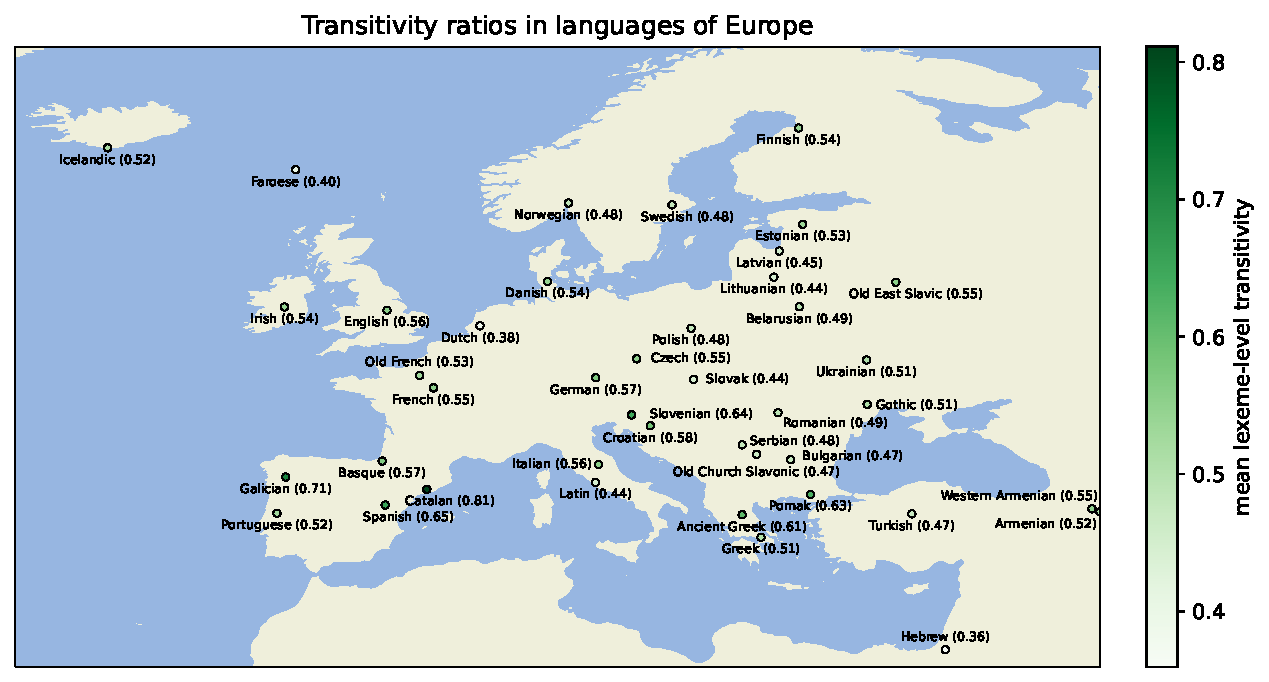
\includegraphics[width=\textwidth]{figures/transitivity_europe.pdf}
  \caption{Mean transitivity ratios in languages of Europe}
  \label{fig:transitivity_europe}
\end{figure}

compare results with \citet{say2014} - same areal patterns

\section{Experiment 2: Valency entropy}
\subsection{Motivation}
\subsection{Experiment design}
\subsection{Results}

\section{Experiment 3: Word order and case information}
\subsection{Motivation}
\subsection{Experiment design: ablation studies}
\subsection{Results}

\section{Experiment 4: Verb entropy}
\subsection{Motivation}
\subsection{Experiment design}
\subsection{Results}

\section{Experiment 5: Verb-finalness}
\subsection{Motivation}
\subsection{Experiment design}
\subsection{Results}